\documentclass[12pt, letterpaper]{report}

\usepackage{graphicx}
\usepackage{subfig}
\usepackage{url}
\usepackage{color}
%\usepackage[justification=justified]{caption}[2009/9/16]
\usepackage[top=1in, bottom=1in, left=1.5in, right=1in]{geometry}
\usepackage{hyperref}

\frenchspacing %same spacing between words and sentences cf. http://en.wikibooks.org/wiki/LaTeX/Formatting#Space_between_Words_and_Sentences

%page numbering--needs to be top right, not yet working
\pagestyle{myheadings}
\markright{\hfill}

\begin{document}

\title{Search in the Two-Photon Final State for Evidence of New Particle Production at the Large Hadron Collider}
\author{Rachel P. Yohay \\
	University of Virginia \\
	\texttt{rpy3y@virginia.edu}}
\date{\today}
\maketitle

\tableofcontents

\chapter{Introduction}
%failures of the Higgs mechanism, dark matter, how SUSY ties them together

\chapter{Overview of the Standard Model of Particle Physics}
%\chapter{The Current State of the Standard Model}

I call it...the Aristocrats.

%The Standard Model of particle physics describes the elementary building blocks of matter as a set of interacting field quanta.  There are four forces by which the quanta, or particles, may interact: the the weak force, electromagnetic force, the strong force, and the gravitational force.  Table 1 lists some properties of the four forces.

%insert table here showing each force, its carrier, and the physical phenomena it applies to
%\begin{tabular}{|l|l|l|}
%\hline
%Force & Associated particle(s) & Physical phenomena \\
%\hline
%\hline
%Weak & $W^{\pm}$ (80.4 $GeV/c$), $Z^{0}$ (91.2 $GeV/c$) & Radioactive $\beta$ decay, fusion in stars \\
%\hline
%Electromagnetic & Photon & Electricity, 
%\end{tabular}

%In addition to the matter particles, there also exist particles associated to each of the forces.  Interactions between matter particles, for instance via scattering or pair production, are mediated by the exchange or creation of virtual force carriers \cite{Cottingham_and_Greenwood}.

In the 1960s, Sheldon Glashow, Steven Weinberg, and Abdus Salam proposed a mathematical framework that unified the electromagnetic and weak forces at an energy scale in the hundreds of GeV/c, as well as a mechanism for breaking the electroweak symmetry at low energies \cite{Glashow_Weinberg_and_Salam}.  At the same time, Murray Gell-Mann introduced the concept of quarks to describe hadron spectroscopy, a concept that would later grow into quantum chromodynamics (QCD), the full theory of the strong force \cite{Gell-Mann}.  These two key developments motivated the unified representation of particle physics as a set of fields whose dynamics are invariant under the Standard Model gauge group

\begin{equation}
SU(3)_{C} \bigotimes SU(2)_{L} \bigotimes U(1)_{EM}
\end{equation}
%
where $SU(3)_{C}$ describes the quark QCD interactions, $SU(2)_{L}$ describes the weak interactions among quarks and leptons, and $U(1)_{EM}$ describes the electromagnetic interaction.

The Standard Model, in particular the electroweak theory, has been an extremely successful predictor of particle production and interaction cross-sections and decay rates, as well as of the exact masses of the electroweak force carriers.  The case for the validity of the Standard Model was bolstered by the many precision QCD and electroweak measurements carried out at the Large Electron-Positron (LEP) collider, which ran from 1989-2000 at center-of-mass energies between 65 and 104 GeV/c \cite{Drees}.  Figure 1 shows some of the highlights of the LEP program.

\begin{figure}
	\centering
	\subfloat[Total hadronic cross-section as a function of collider center-of-mass energy.]{\label{fig:LEP_hadronic_xsec}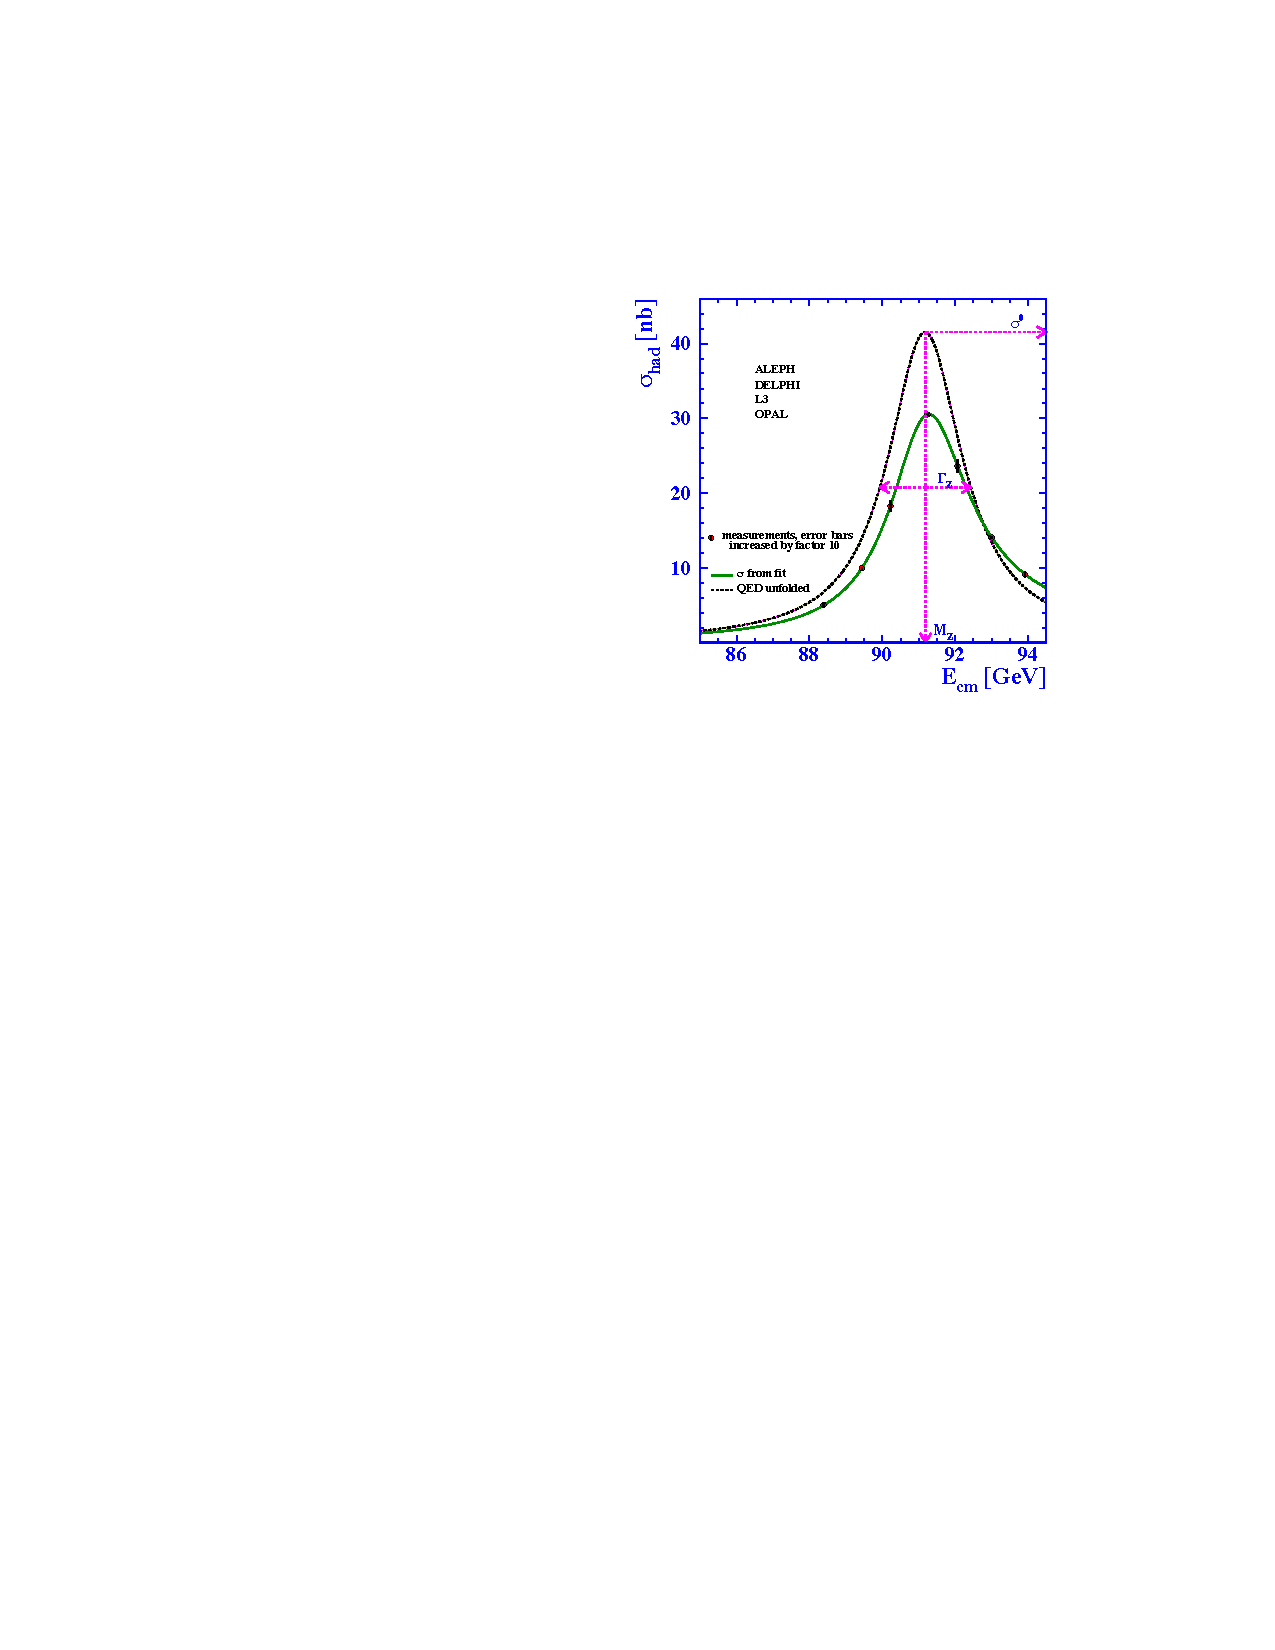
\includegraphics[scale=0.7]{LEP_hadronic_xsec}}
	\hspace{1cm}
	\subfloat[Measured and predicted dependence of the $q\overline{q}$, $\mu^{+}\mu^{-}$, and $\tau^{+}\tau^{-}$ pair production cross sections on LEP center-of-mass energy.]{\label{fig:LEP_pair_production_xsecs}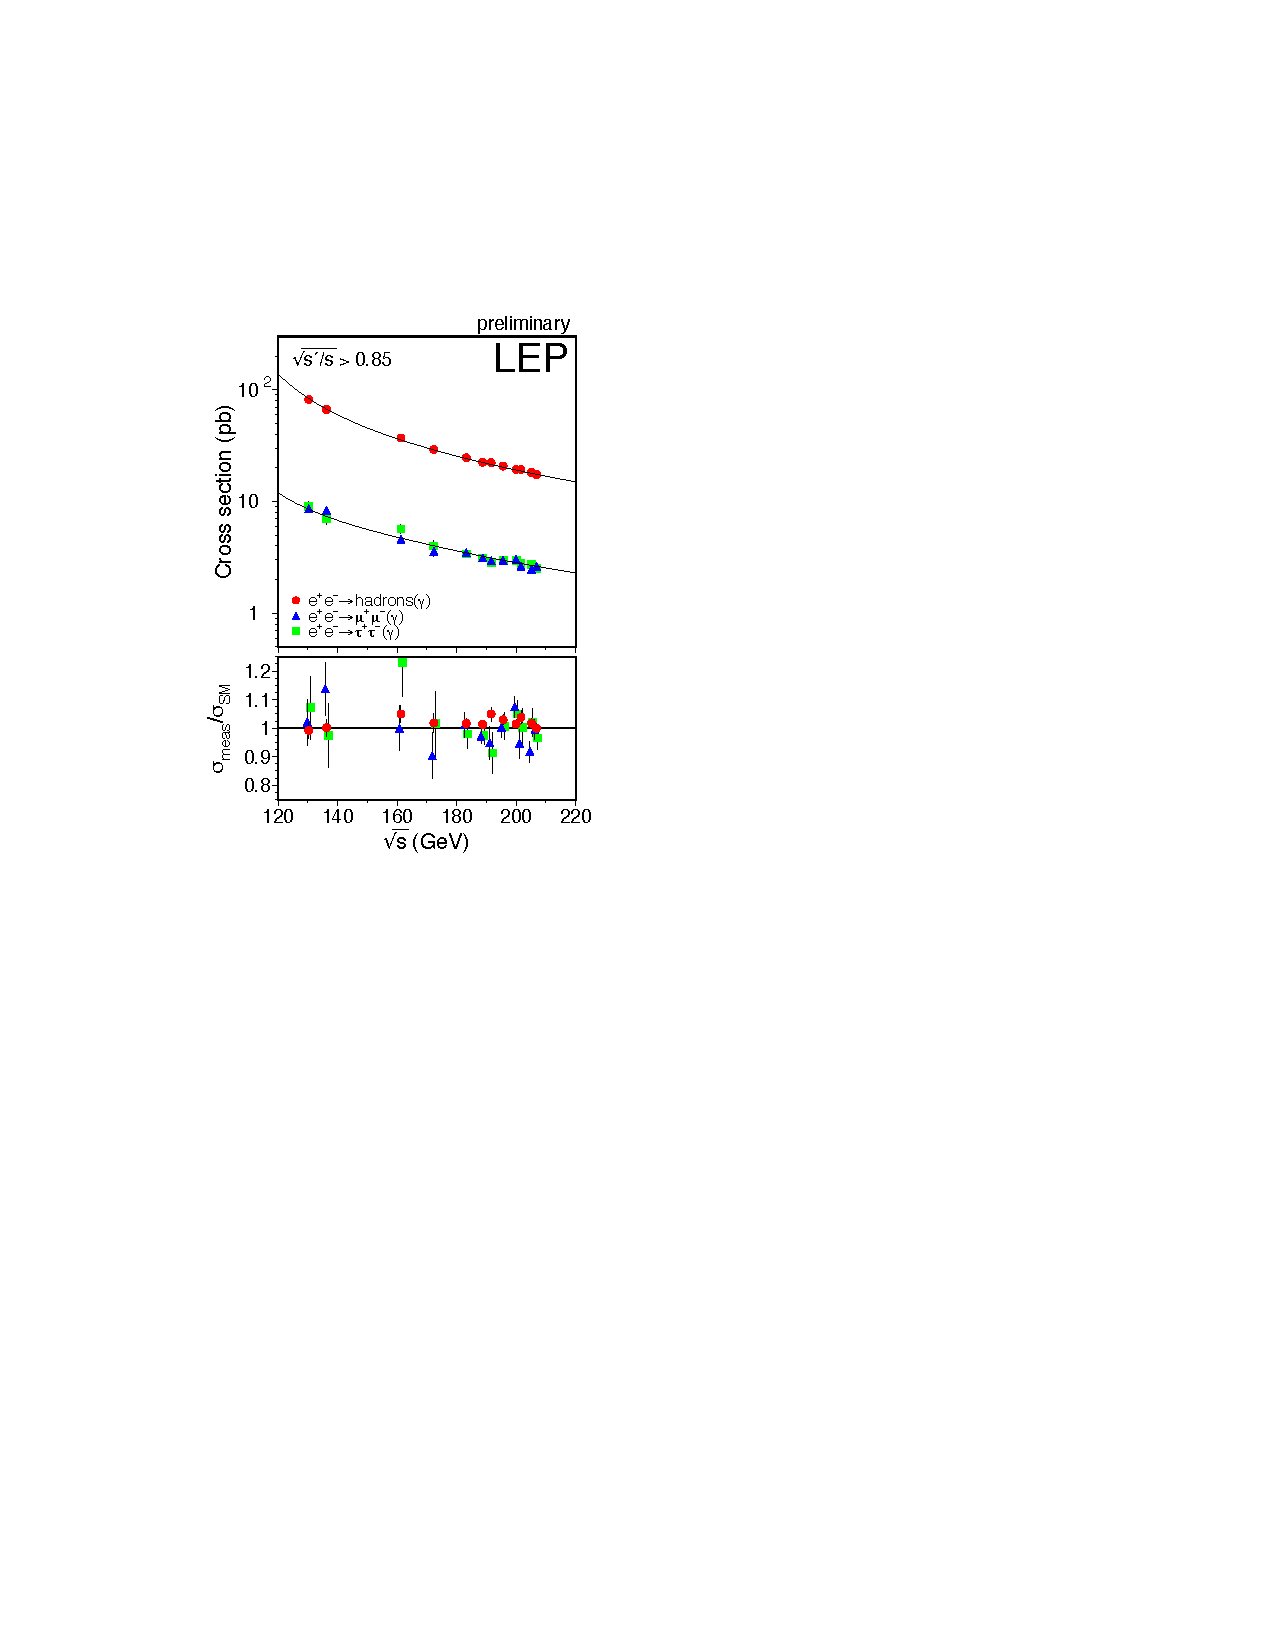
\includegraphics[scale=0.7]{LEP_pair_production_xsecs}}
	\\
	\subfloat[Measured and predicted dependence of the $W^{+}W^{-}$ pair production cross section on LEP center-of-mass energy.]{\label{fig:LEP_W_pair_production_xsec}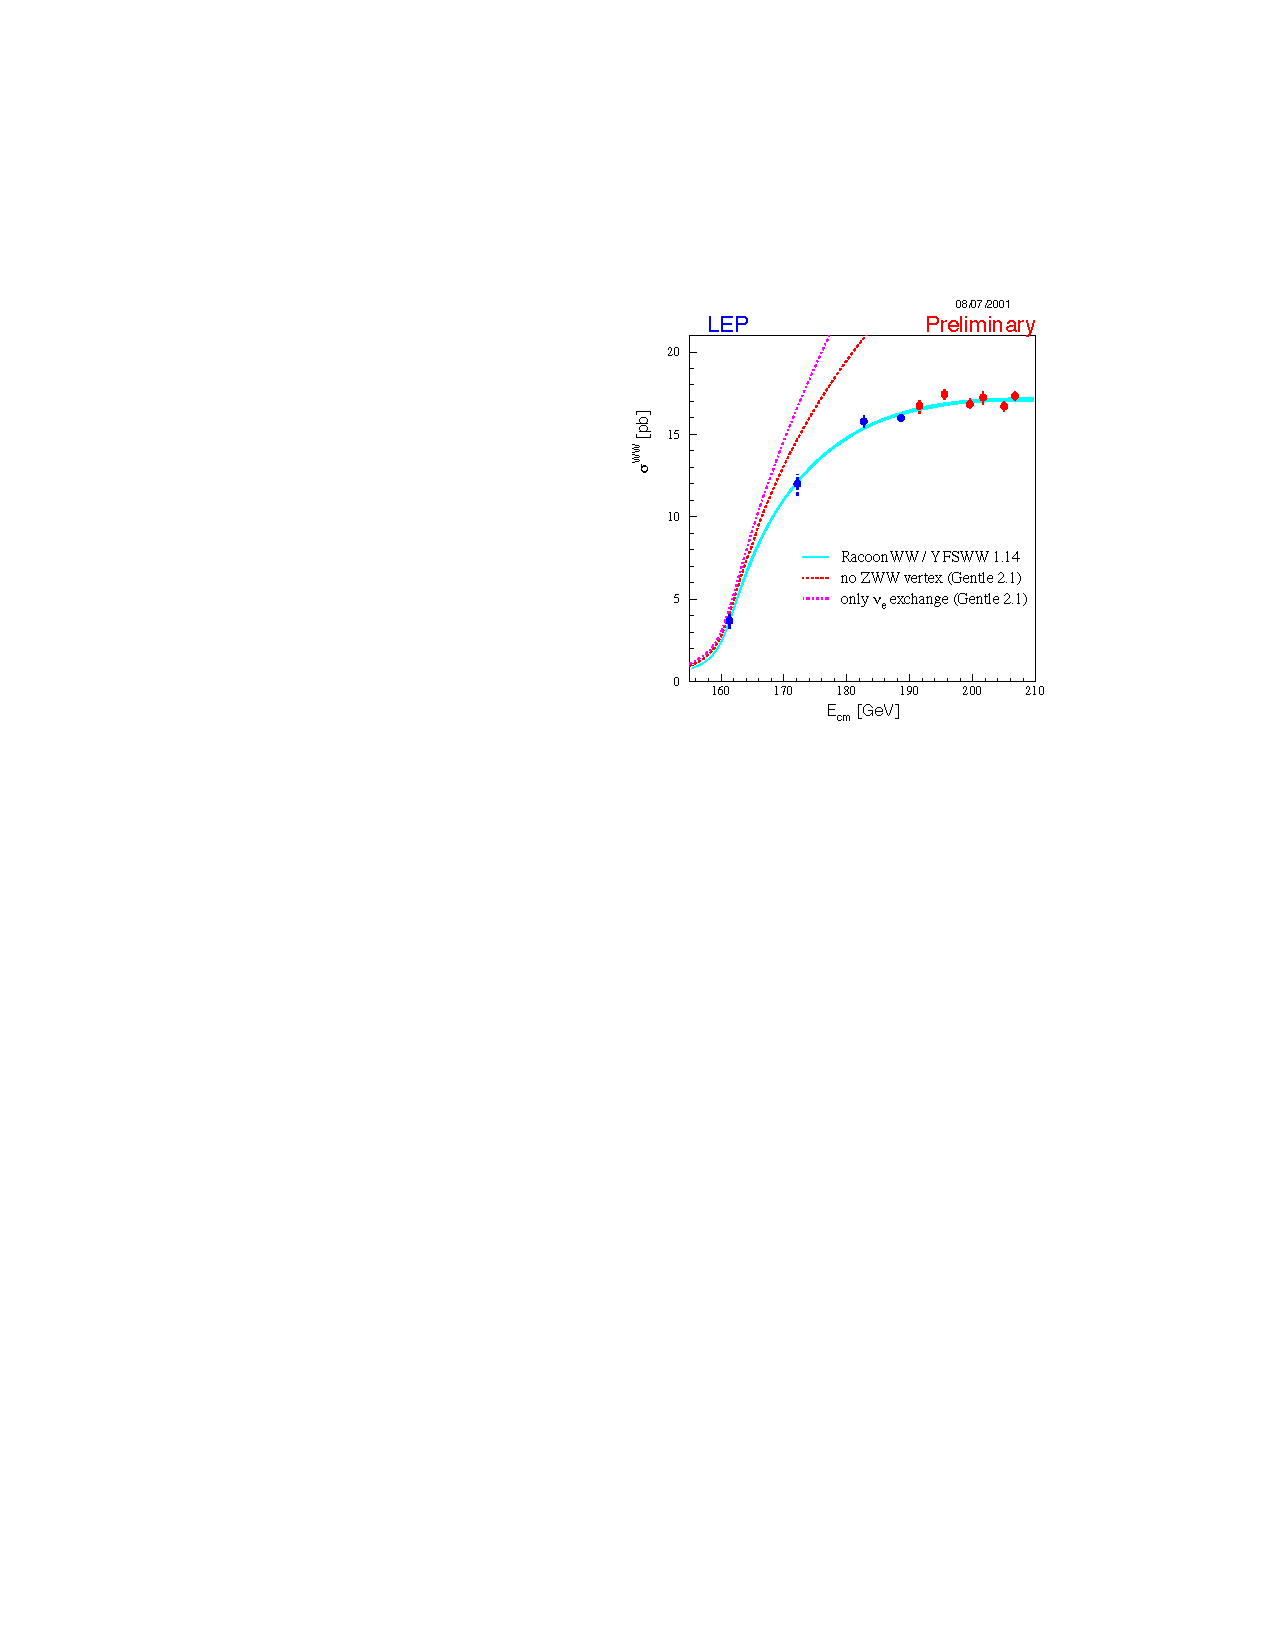
\includegraphics[scale=0.7]{LEP_W_pair_production_xsec}}
	\hspace{1cm}
	\subfloat[Measured and predicted dependence of the strong coupling constant $\alpha_{s}$ on LEP center-of-mass energy.]{\label{fig:LEP_alphaS_running}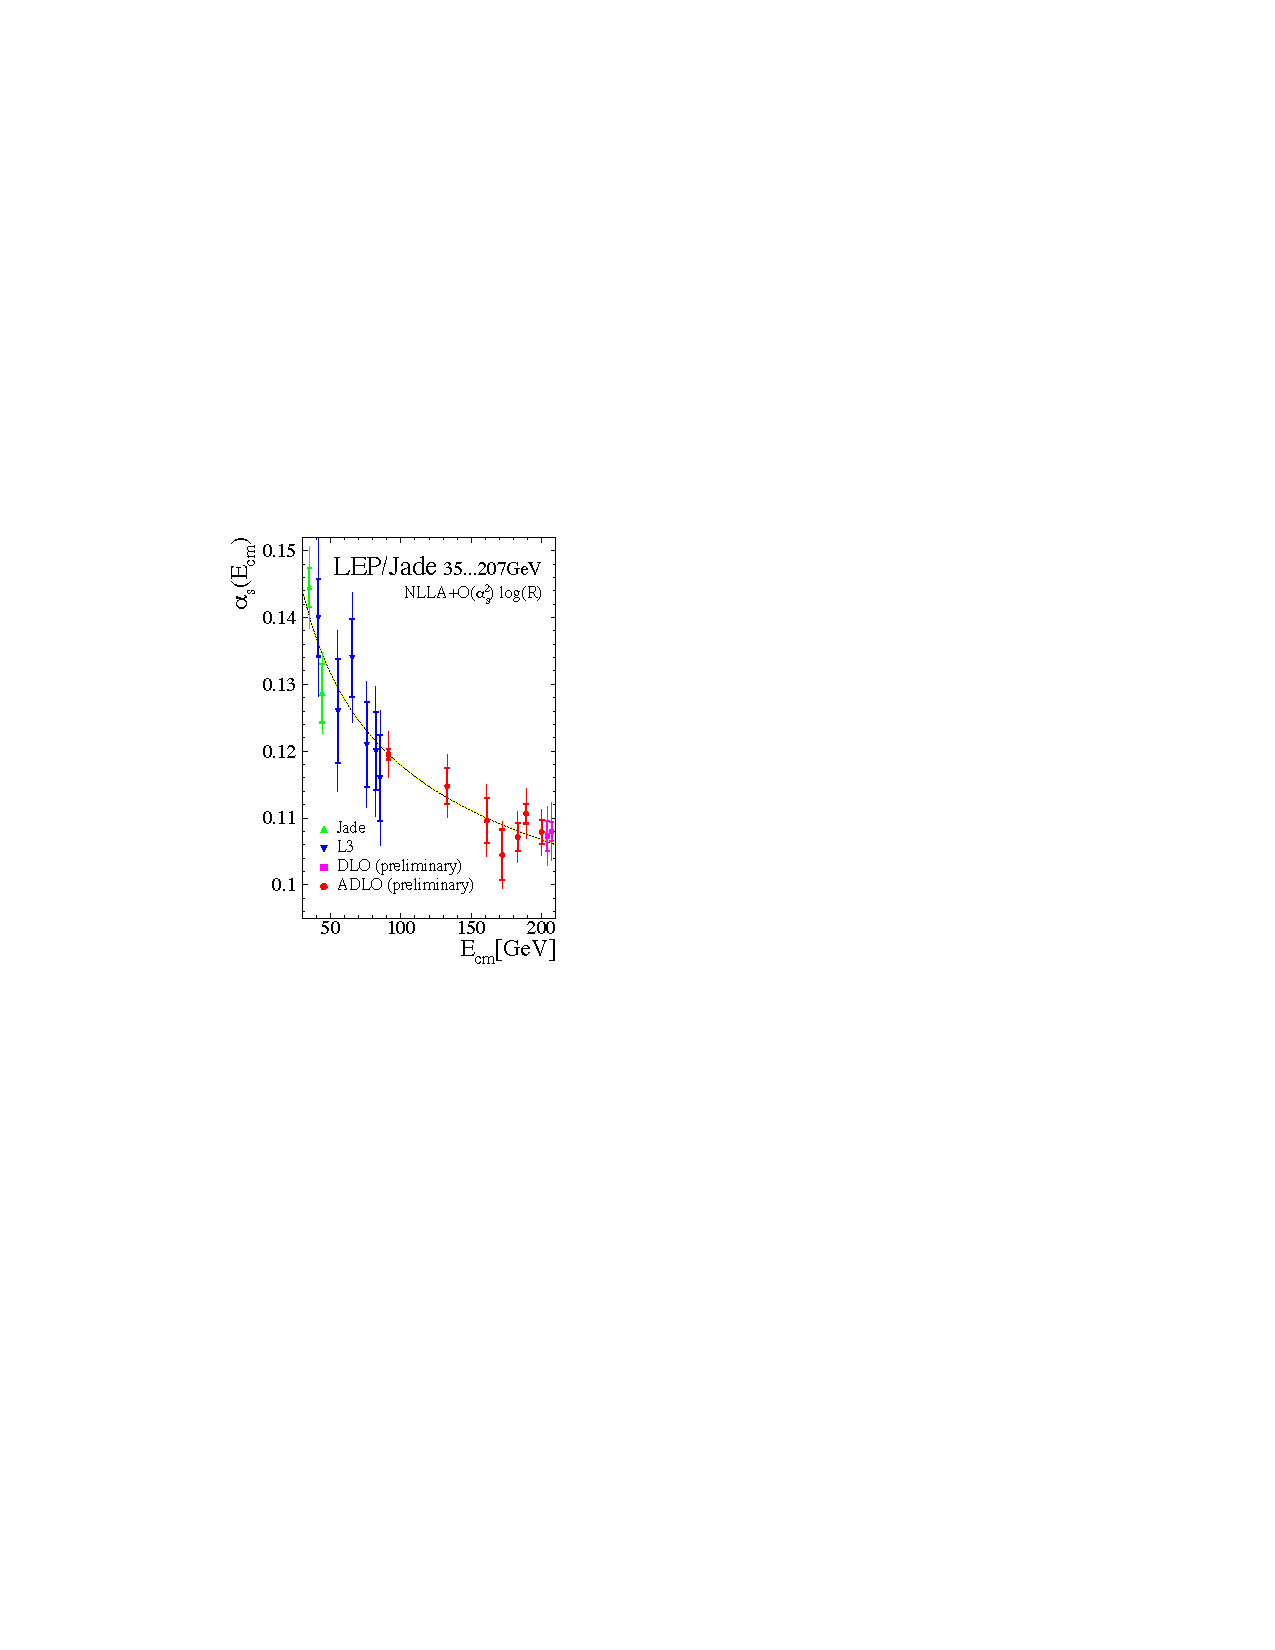
\includegraphics[scale=0.7]{LEP_alphaS_running}}
	\label{fig:LEP}
	\caption{Selected LEP measurements demonstrating its contribution to the precise understanding of the Standard Model.  Reprinted from \cite{Drees}.}
\end{figure}

However, there are still deep theoretical problems with the Standard Model, stemming from the introduction of the Higgs scalar into the theory to break electroweak symmetry \cite{Higgs}.  Since the Higgs self-energy diagram is quadratically sensitive to the ultraviolet cutoff scale(footnote: this is a general property of scalar fields), and assuming that there are no new important energy scales of physics between the weak scale ($\mathcal{O}$($10^{2}$ GeV/c)) and the Planck scale ($\mathcal{O}$($10^{19}$ GeV/c)), in order to be consistent with experimental measurements, this diagram must include a remarkable 17-orders-of-magnitude cancellation that is otherwise poorly motivated \cite{Aitchison}.  The quest to find new physics at an intermediate energy scale between the weak and Planck scales, and thus extend the Standard Model, was the driving force behind the construction of the Large Hadron Collider (LHC) in 2009, the world's highest energy particle accelerator to date.

In this chapter I will briefly describe the Standard Model particle content, the theory and major results of electroweak symmetry breaking (EWSB), and the problems that the Standard Model is as yet ill-prepared to address.

\section{Particle Content}
%group theory representation
%doublets, singlets, charges
%masses: why so different?
%Fermi vs. Bose statistics
\section{Electroweak Symmetry Breaking and the Higgs Mechanism}
\section{The Hierarchy Problem, The Origins of Mass, and Fine Tuning}

\chapter{The Supersymmetric Extension to the Standard Model}
\section{SUSY Lagrangian and Particle Content, SUSY Breaking}
\section{Dark Matter and the WIMP Miracle}
\section{Gauge-Mediated SUSY Breaking}
%minimal
%general -- also describe bino-like vs. wino-like in terms of M1 and M2, say it will be important later
%phenomenological differences
\section{Experimental Status of SUSY}

Collider searches for evidence of supersymmetry began in earnest in the 1980s (\cite{SUSY_history}) and continue to this day.  Most recently, the LHC and Tevatron\footnote{Located on the Fermilab site in Batavia, Illinois, the Tevatron was a proton-antiproton collider operating at 1.96 TeV center-of-mass energy.  The Tevatron ran from 1987 to 2011 \cite{Tevatron_lifetime}.} experiments have set the strictest limits on a variety of SUSY breaking scenarios, including GMSB and mSUGRA (discussed below).

Figure X shows the current limits set by the CMS experiment on the mSUGRA model (with tan $\beta$ = 10) in the $m_{0}$-$m_{1/2}$ plane.  (Note that although the plot is truncated at $m_{0}$ = 1000 GeV/$\mbox{c}^{2}$, some searches are sensitive out to $m_{0} \sim$ 2000 GeV/$\mbox{c}^{2}$.)  Although the LHC has pushed $m_{0}$ above $\sim$1 TeV/$\mbox{c}^{2}$ for $m_{1/2}$ up to $\sim$400 GeV/$\mbox{c}^{2}$, casting some doubt onto the theory's prospects for solving the hierarchy problem, there is still a sizable chunk of mSUGRA parameter space that is not ruled out by collider experiments.  Furthermore, parts of the CMS unexplored regions overlap with areas allowed by astrophysics experiments \cite{CMSSM_fits}.

\begin{figure}
	\centering
	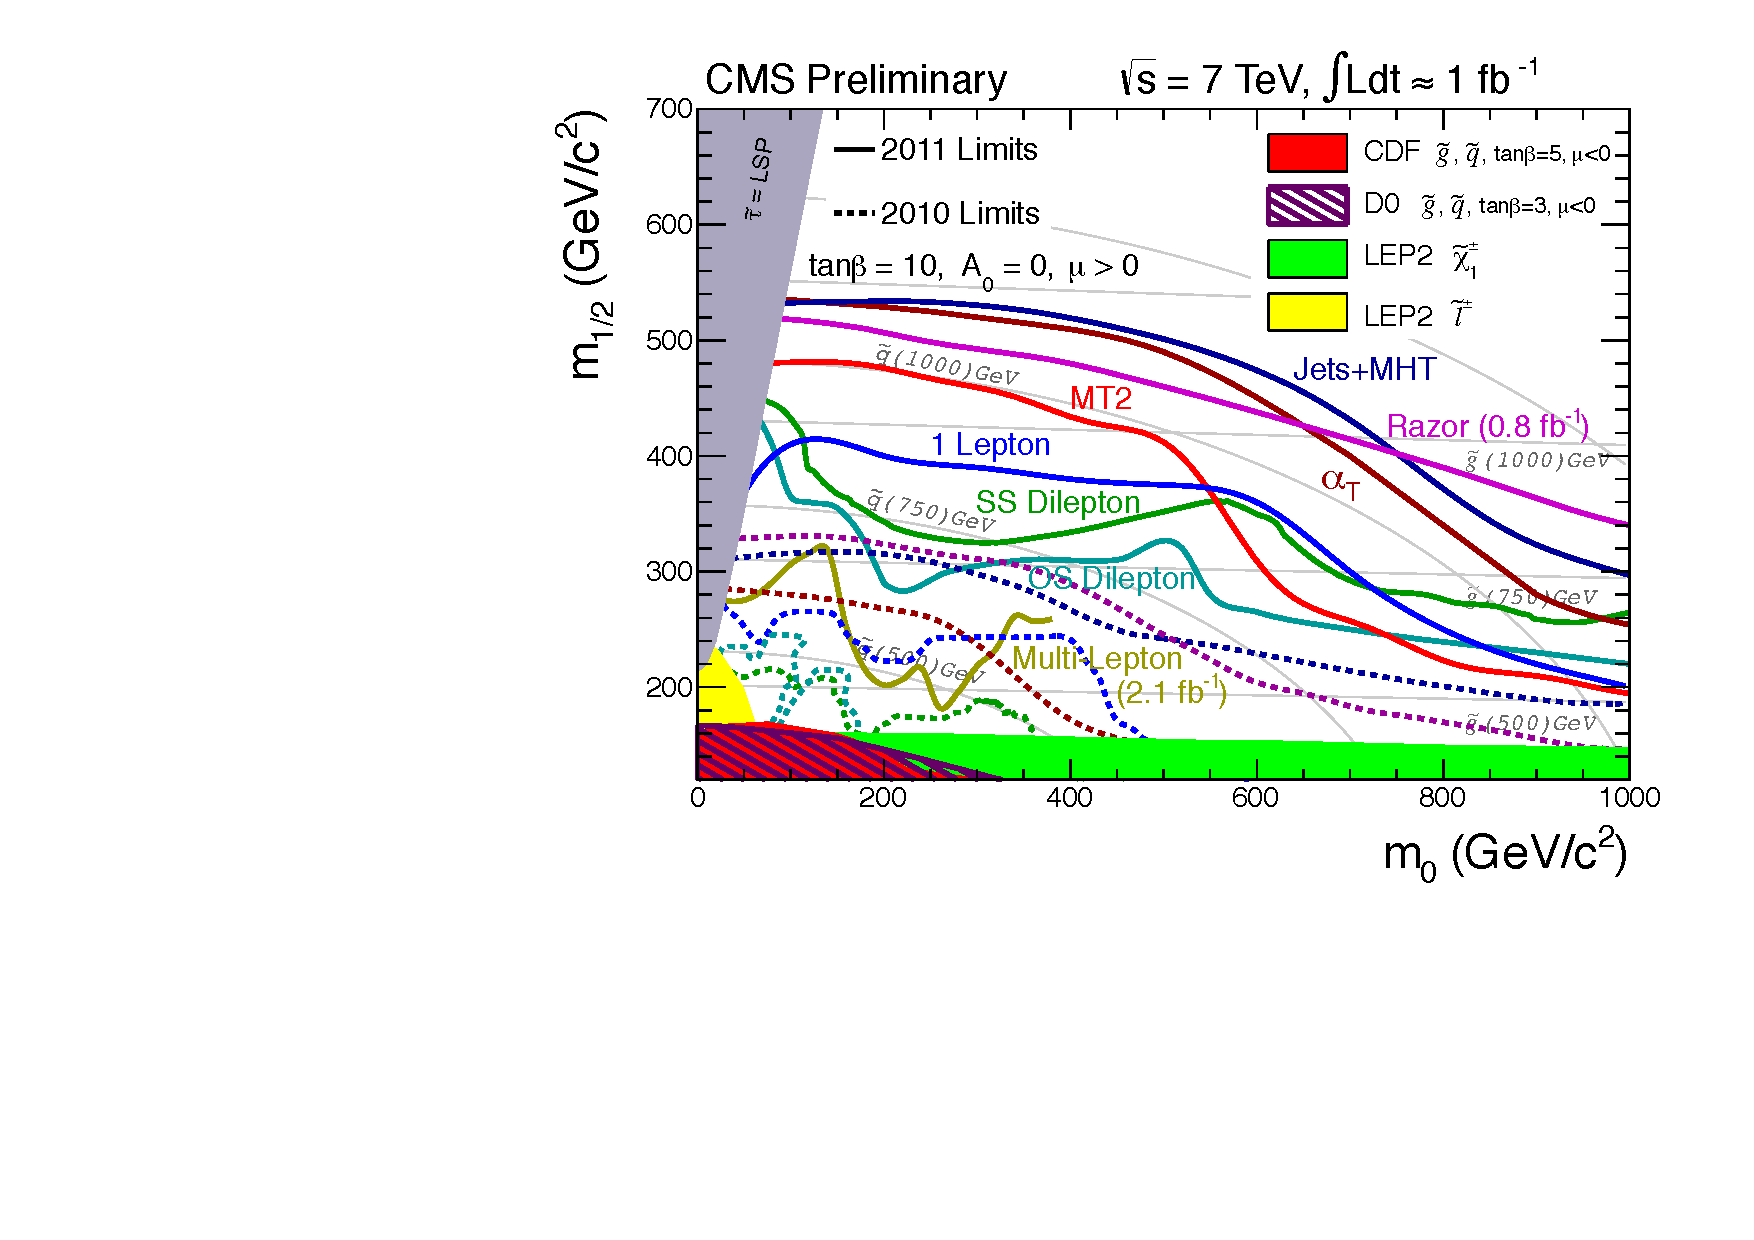
\includegraphics[scale=0.6]{CMS_SUSY_2011Limits_tanb10}
	\caption{CMS limits on mSUGRA with tan $\beta$ = 10.  The limits set by individual searches are shown as separate colored lines.  Solid lines refer to 2011 searches (i.e. using an integrated luminosity of $\sim$1 $\mbox{fb}^{-1}$), while dashed lines refer to 2010 searches ($\sim$36 $\mbox{pb}^{-1}$).  Reprinted from \cite{CMS_mSUGRA}.}
\end{figure}

%check the whole next paragraph and figures from ATLAS!

Figure X shows the most up-to-date limit (using 1 $\mbox{fb}^{-1}$ of integrated luminosity collected by the ATLAS experiment \cite{ATLAS} at the LHC) on the Snowmass Points and Slopes (SPS) model of minimal GMSB (mGMSB), dubbed SPS8 \cite{SPS}.  SPS8 represents the simplest class of GMSB models described in Sec. X.  The best limits on a variety of general gauge mediation (GGM) models, from the same ATLAS study, are shown in Figure X.  In these models, no assumptions are made about the specific parameters common to many gauge mediation models (e.g. the number of messengers or the relationship between the messenger mass and the SUSY breaking scale).  Instead, it is only assumed that the lightest neutralino is light enough to be produced on-shell at the LHC (by setting $\mbox{M}_{1}$ and $\mbox{M}_{2}$ appropriately, see Sec. X) and that it decays to a gravitino, that the gravitino is extremely relativistic (mass of order eV-keV), and that the gravitino is stable.  The one-dimensional scan over SUSY breaking scales in the SPS8 model (in which the full sparticle spectrum is specified by the model parameters) is replaced by a two-dimensional scan over gluino and lightest neutralino mass in the GGM models (in which all sparticles except the gluino, first- and second-generation squarks, and neutralinos are forced to be at $\sim$1.5 TeV/$\mbox{c}^{2}$, effectively decoupling them from the dynamics that can be probed with 1 $\mbox{fb}^{-1}$ at a 7 TeV/c pp collider).  %maybe repeat some of this in the earlier section about the advantages of simplified models (can make a more logical, clear mapping between search strategy and model sensitivity, can be less model-dependent)

\begin{figure}
	\centering
	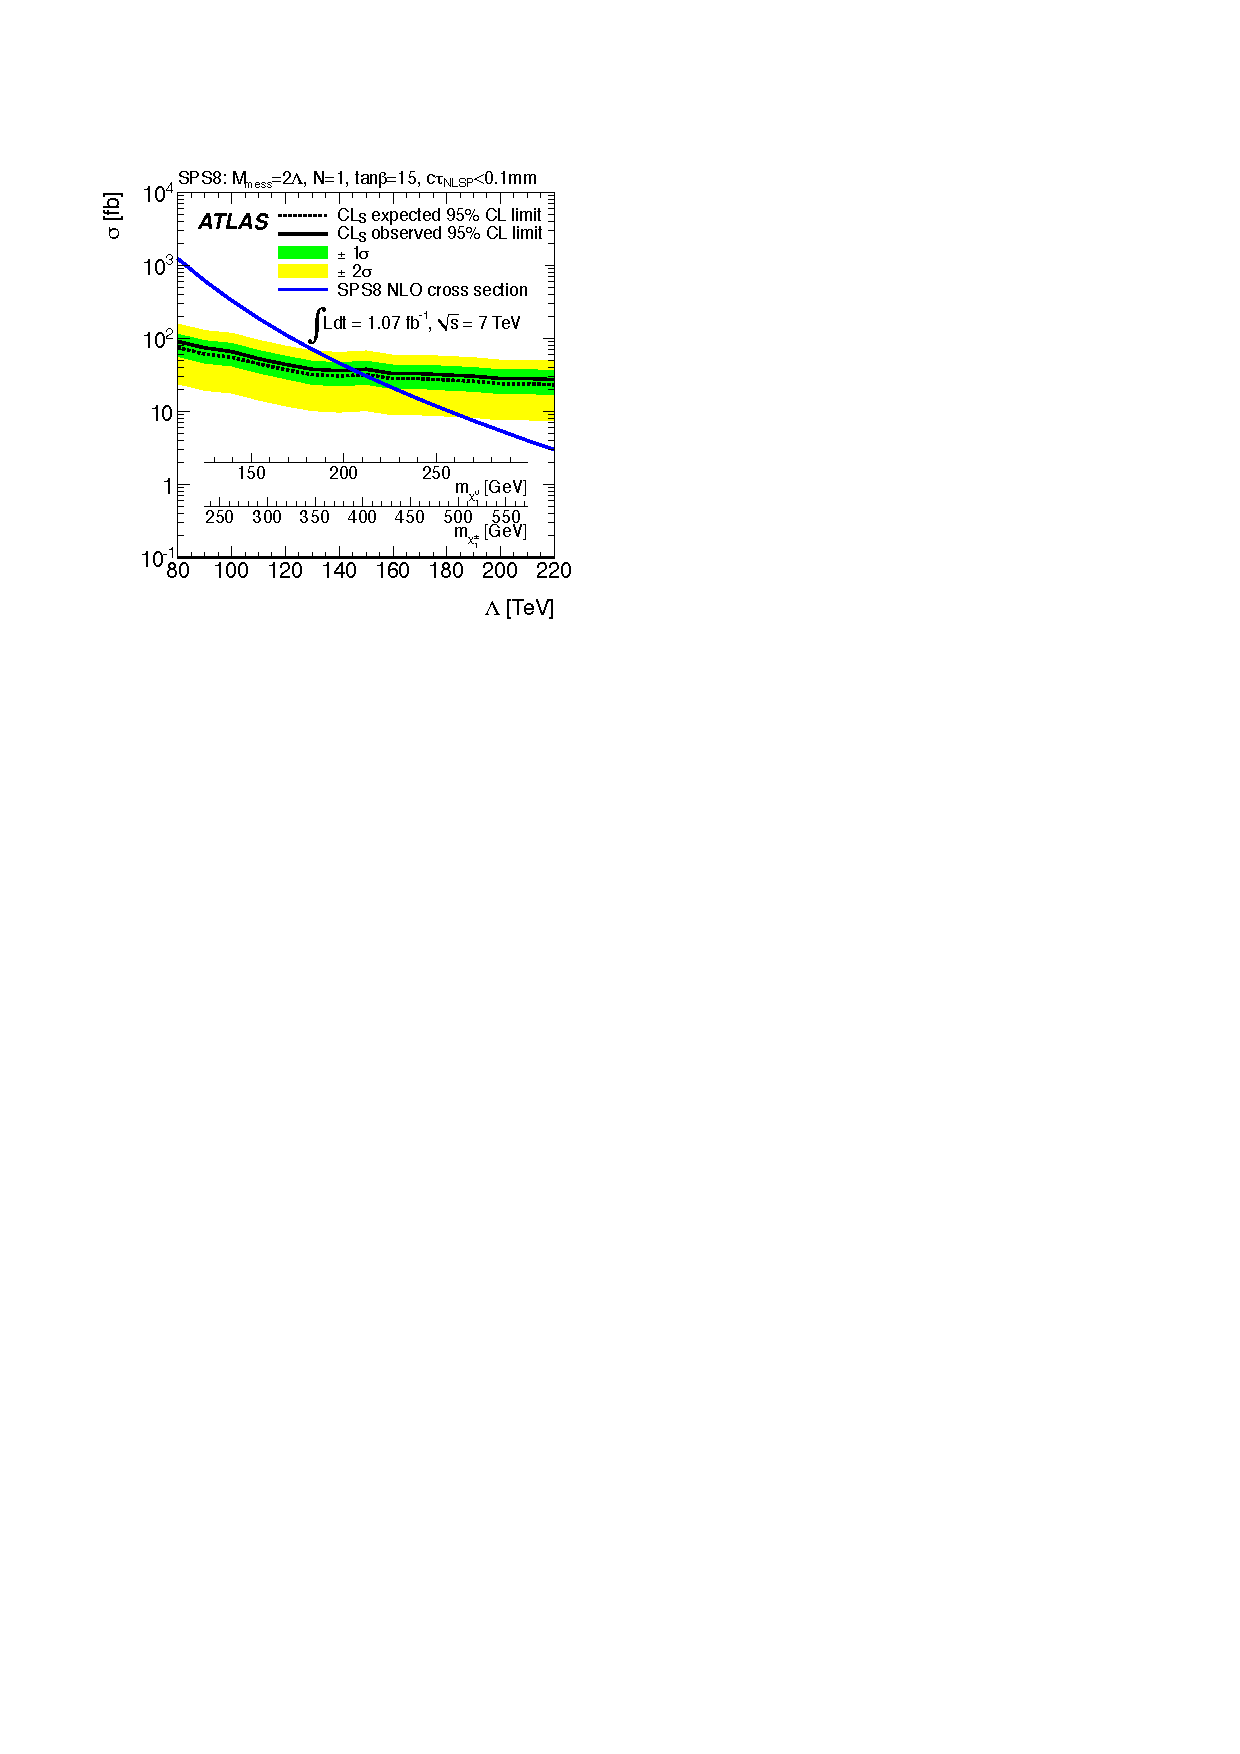
\includegraphics[scale=0.9]{ATLAS_SPS8_limit}
	\caption{ATLAS cross section upper limit on the SPS8 \cite{SPS} model of mGMSB as a function of SUSY breaking scale $\Lambda$, lightest neutralino mass $m_{\widetilde{\chi}_{1}^{0}}$, or lightest chargino mass $m_{\widetilde{\chi}_{1}^{\pm}}$.  Values of $\Lambda$, $m_{\widetilde{\chi}_{1}^{0}}$, or $m_{\widetilde{\chi}_{1}^{\pm}}$ below the intersection point between the blue (predicted SPS8 cross section) and black (observed cross section upper limit) curves are excluded.  The model parameters listed above the plot are defined in Sec. X.  Reprinted from \cite{ATLAS_GMSB_1fb-1}.}
\end{figure}

\begin{figure}
	\centering
	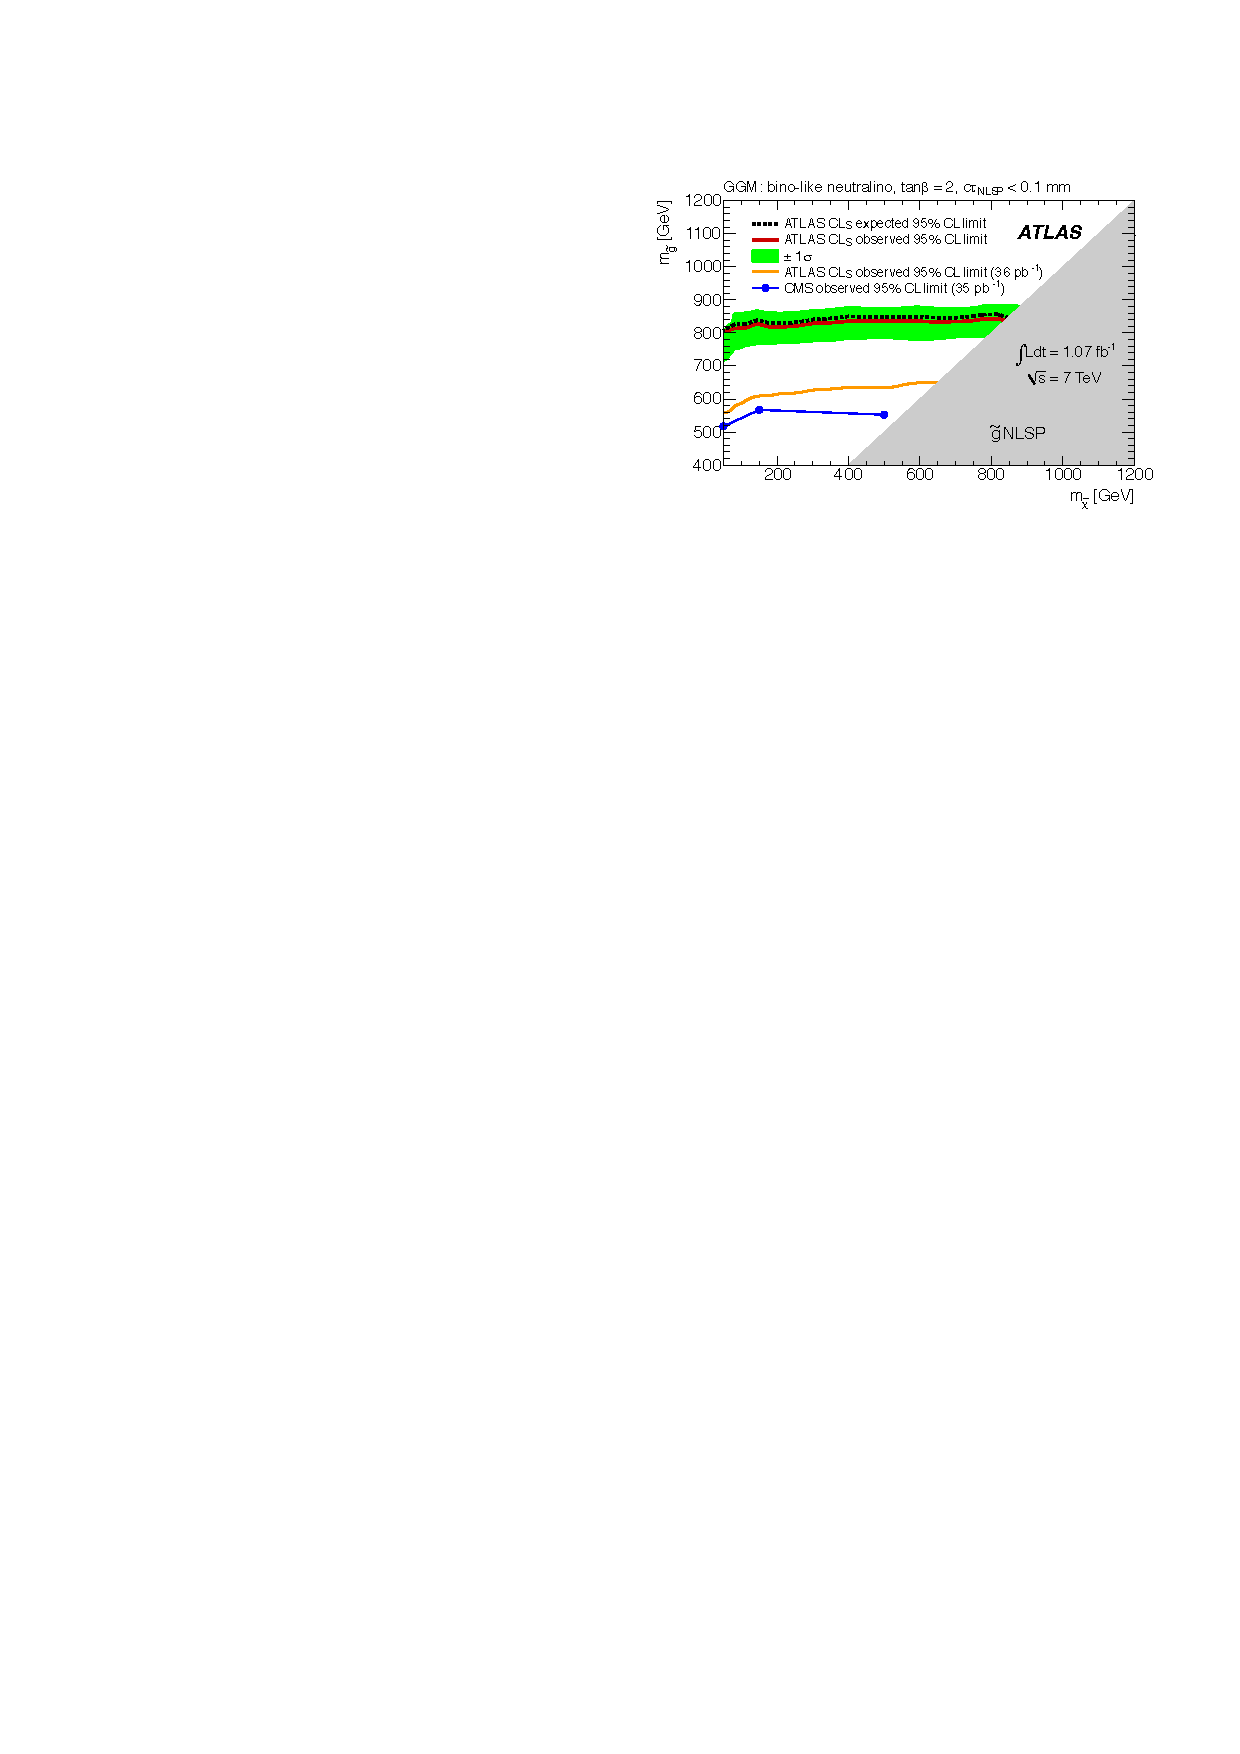
\includegraphics[scale=0.9]{ATLAS_GGM_limit}
	\caption{ATLAS exclusion contour in the $m_{\widetilde{g}}$-$m_{\widetilde{\chi}}$ plane.  Values of $m_{\widetilde{g}}$-$m_{\widetilde{\chi}}$ below the red curve are excluded.  The gray region is theoretically excluded in the GGM models considered.  "Bino-like neutralino" means that $\mbox{M}_{2}$ = 1.5 TeV/$\mbox{c}^{2}$.  Reprinted from \cite{ATLAS_GMSB_1fb-1}.}
\end{figure}

In general, the lifetime of the lightest neutralino in GMSB models can take on any value between hundreds of nanometers to a few kilometers depending on the mass of the lightest neutralino and the SUSY breaking scale \cite{SUSY_primer}.  The search published in \cite{ATLAS_GMSB_1fb-1} (from which Figs. X and X are culled) considers only \textit{prompt} neutralino variants, i.e. with neutralino lifetime short enough that the distance traveled by the neutralino before decay cannot be resolved by the detector.  The most recent limits on non-prompt neutralino models were set by the Collider Detector at Fermilab (CDF) collaboration with X $\mbox{fb}^{-1}$, and are shown in Figure X.

%and now go into long-lived NLSPs--motivation from cosmology?

Table X summarizes the current best limits on the GMSB scenarios discussed in this section.

%CDF/D0 long-lived

%astrophysics exclusions

\chapter{The Large Hadron Collider}
%see LHC paper
%injection chain, energy, RF, focusing, beam structure, luminosity increases, pileup

\chapter{The Compact Muon Solenoid Experiment}
%see detector paper
%overview, pointing out CMS on the ring, coordinate system and theta, eta, phi, ET, pT, etc. definition
%picture of the cross-section
\section{The Detectors and Their Operating Principles}
\subsection{Tracking System}
\subsubsection{Pixel Detector}
\subsubsection{Silicon Strip Tracker}
\subsection{Electromagnetic Calorimeter}
%make this big, include EE work
\subsection{Hadronic Calorimeter}
\subsection{Muon System}
%spend very little time on this
\subsection{Far Forward Calorimetry}
%spend very little time on this
\section{Triggering, Data Acquisition, and Data Transfer}
\subsection{Level 1 and High Level Trigger Systems}
\subsection{Data Acquisition System}
\subsection{Data Processing and Transfer to Computing Centers}

\chapter{Event Selection}
%2 photons + MET
\section{HLT}
\section{Object Reconstruction}
\subsection{Photons}
\subsection{Electrons}
\subsection{Jets and Missing Transverse Energy}
\section{Photon Identification Efficiency}

\chapter{Data Analysis}
%look for high MET excess
%main backgrounds, justify the negligible ones
\section{Modeling the QCD Background}
\section{Modeling the Electroweak Background}
\section{Results}
%including all uncertainties

\chapter{Interpretation of Results in Terms of GMSB Models}
\section{Simplified Models}
%signal uncertainties, scale factor stuff, MC parameters 
\section{Upper Limit Calculation}
\section{Cross Section Upper Limits}
\section{Exclusion Contours}

\chapter{Conclusion}

\begin{thebibliography}{99}
%\bibitem{Cottingham_and_Greenwood} dummy
\bibitem{Glashow_Weinberg_and_Salam} S.L. Glashow, J. Iliopoulis, and L. Maiani, \textit{Phys. Rev. D} \textbf{2} (1970) 1285; S.L. Glashow, \textit{Nucl. Phys.} \textbf{22(4)} (1961) 579; J. Goldstone, A. Salam, and S. Weinberg, \textit{Phys. Rev.} \textbf{127} (1962) 965; S. Weinberg, \textit{Phys. Rev. Lett.} \textbf{19} (1967) 1264; A. Salam and J.C. Ward, \textit{Phys. Lett.} \textbf{13(2)} (1964) 168.
\bibitem{Gell-Mann} M. Gell-Mann, \textit{Phys. Lett.} \textbf{8} (1964) 214; G. Zweig, \textit{CERN} \textbf{8419/TH. 412} (1964) (unpublished).
\bibitem{Drees} J. Drees, \textit{Int. J. Mod. Phys.} \textbf{A17} (2002) 3259.
\bibitem{Higgs} P.W. Higgs, \textit{Phys. Lett.} \textbf{12(2)} (1964) 132; P.W. Higgs, \textit{Phys. Rev. Lett.} \textbf{13} (1964) 508; P.W. Higgs, \textit{Phys. Rev.} \textbf{145} (1966) 1156.
\bibitem{Aitchison} I. Aitchison, \textit{Supersymmetry in Particle Physics: An Elementary Introduction} (Cambridge University Press, Cambridge 2007), p. 4.
\bibitem{SUSY_history} E. Fernandez et al., \textit{Phys. Rev. Lett.} \textbf{54} (1985) 1118; E. Fernandex et al., \textit{Phys. Rev.} \textbf{D35} (1987) 374; D. Decamp et al., \textit{Phys. Lett.} \textbf{B237(2)} (1990) 291; F. Abe et al., \textit{Phys. Rev. Lett.} \textbf{75} (1995) 613; S. Abachi et al., \textit{Phys. Rev. Lett.} \textbf{75} (1995) 618; G. Alexander et al., \textit{Phys. Lett.} \textbf{B377(4)} (1996) 273; S. Aid et al., \textit{Z. Phys.} \textbf{C71(2)} (1996) 211; S. Aid et al., \textit{Phys. Lett.} \textbf{B380(3-4} (1996) 461; B. Aubert et al., \textit{Phys. Rev. Lett.} \textbf{95} (2005) 041802.
\bibitem{Tevatron_lifetime} \url{http://en.wikipedia.org/wiki/Tevatron}.
\bibitem{CMSSM_fits} O. Buchmueller et al., \textit{CERN-PH-TH/2011-220} (2011).
\bibitem{CMS_mSUGRA} \url{https://twiki.cern.ch/twiki/bin/view/CMSPublic/PhysicsResultsSUS}.
\bibitem{ATLAS} G. Aad et al., \textit{JINST} \textbf{3} (2008) S08003.
\bibitem{SPS} B.C. Allanach et al., \textit{Eur. Phys. J.} \textbf{C25} (2002) 113.
\bibitem{ATLAS_GMSB_1fb-1} G. Aad et al., \textit{CERN-PH-EP-2011-160} (2011).
%how to do this citation?
\bibitem{SUSY_primer} S. P. Martin, \textit{A Supersymmetry Primer} \textbf{v4} (2006) 86.  \href{http://arxiv.org/abs/hep-ph/9709356}{arXiv:hep-ph/9709356}.
\end{thebibliography}

\end{document}